\documentclass[11pt, addpoints, answers]{exam}

\usepackage{amsmath, amssymb}
\usepackage{xcolor}

\newcommand{\red}[1]{\textcolor{red}{#1}}

% For inserting code snippets.
\usepackage{listings}
\lstset{
    columns = fixed,
    basewidth = {0.5em},
    breaklines = true,
    backgroundcolor = \color{white},
    keywordstyle = \color[RGB]{40, 40, 255},
    numberstyle = \footnotesize\color{darkgray},
    commentstyle = \ttfamily\color{violet},
    basicstyle = \ttfamily,
    stringstyle = \ttfamily\color[RGB]{128, 0, 0},
    showstringspaces = false,
    language = {[11]C++},
    escapechar = \@
}
\lstnewenvironment{cpp}[1][]{\lstset{language = {[11]C++}, #1}}{}

\usepackage{tikz}
\usepackage{tikz-qtree}


% headers, footers, titles
\newcommand{\CourseName}{CS101 Algorithms and Data Structures}
\newcommand{\HomeworkNO}{Homework 6}
\newcommand{\DueDate}{Due date: November 19, 2023, at 23:59}

\pagestyle{headandfoot}
\runningheadrule
\runningheader{\CourseName}{\HomeworkNO}{\DueDate}
\runningfooter{}{\thepage}{}

\title{
	\CourseName\\
	Fall 2023\\
	\HomeworkNO
}
\author{}
\date{\DueDate}

% formats of questions, choices, points, etc.
\qformat{\bf\thequestion. (\totalpoints\ points) \thequestiontitle\hfill}
\pointname{'}
\CorrectChoiceEmphasis{\bf\color{blue}}
\SolutionEmphasis{\color{blue}}

% We frequently use this font.
\newcommand{\ttt}{\texttt}
\newcommand{\bluett}[1]{\textcolor{blue}{\ttt{#1}}}

\begin{document}

\maketitle

\begin{enumerate}
	\item Please write your solutions in English.
	\item Submit your solutions to gradescope.com.
	\item Set your FULL name to your Chinese name and your STUDENT ID correctly in Account Settings.
	\item If you want to submit a handwritten version, scan it clearly. \ttt{CamScanner} is recommended.
	\item When submitting, match your solutions to the problems correctly.
	\item No late submission will be accepted.
	\item Violations to any of the above may result in zero points.
\end{enumerate}

\begin{questions}

\newpage

\titledquestion{Multiple Choices}

Each question has \textbf{one or more} correct answer(s). Select all the correct answer(s). For each question, you will get 0 points if you select one or more wrong answers, but you will get 1 point if you select a non-empty subset of the correct answers.

Write your answers in the following table.

%%%%%%%%%%%%%%%%%%%%%%%%%%%%%%%%%%%%%%%%%%%%%%%%%%%%%%%%%%%%%%%%%%%%%%%%%%%
% Note: The `LaTeX' way to answer a multiple-choices question is to replace `\choice'
% with `\CorrectChoice', as what you did in the first question. However, there are still
% many students who would like to handwrite their homework. To make TA's work easier,
% you have to fill your selected choices in the table below, no matter whether you use 
% LaTeX or not.
%%%%%%%%%%%%%%%%%%%%%%%%%%%%%%%%%%%%%%%%%%%%%%%%%%%%%%%%%%%%%%%%%%%%%%%%%%%

\begin{table}[htbp]
    \centering
    \begin{tabular}{|p{2cm}|p{2cm}|p{2cm}|}
        \hline
        (a) & (b) & (c)                \\
        \hline
        %%%%%%%%%%%%%%%%%%%%%%%%%%%%%%%%%%%%%%%%%%%%%%%%%%%%%%%%%%
        % YOUR ANSWER HERE.
        ABD & ACD & ABC \vspace{0.4cm} \\
        %%%%%%%%%%%%%%%%%%%%%%%%%%%%%%%%%%%%%%%%%%%%%%%%%%%%%%%%%%
        \hline
    \end{tabular}
\end{table}

\begin{parts}

    \part[2] Which of the following statements about Dijkstra's algorithm is/are true?

    \begin{choices}
        \CorrectChoice Once a vertex is marked as visited, its distance will never be updated.
        \CorrectChoice The time complexity of Dijkstra's algorithm using complete binary heap is $\Theta(|E|\log |V|)$.
        \choice If we use Dijkstra's algorithm to find the distance from vertex $s$ to vertex $t$, then when we first push $t$ into the heap, we find the shortest path from $s$ to $t$ and stop the algorithm.
        \CorrectChoice If vertex $u$ is marked visited before $v$, then $\texttt{dist[u]}\le \texttt{dist[v]}$.
    \end{choices}

    \part[2] Which of the following statements about A* search algorithm is/are true?

    \begin{choices}
        \CorrectChoice If we use heuristic function $h(u)=c$ for any $u\in V$ where $c$ is a positive constant, then the A* search algorithm will be the same with Dijkstra's algorithm.
        \choice An admissible heuristic function ensures optimality of both A* tree search algorithm and A* graph search algorithm.
        \CorrectChoice A consistent heuristic function ensures optimality of both A* tree search algorithm and A* graph search algorithm.
        \CorrectChoice Suppose we want to search for the shortest path from a city to another on a map. If we use the heuristic function $h(u)=dis(u,t)$, the Euclidean distance between $u$ and the destination $t$, then this is a consistent heuristic function.
    \end{choices}

    \part[2] Which of the following statements about Bellman-Ford algorithm is/are true?

    \begin{choices}
        \CorrectChoice In a DAG with probably negative edge weights, Bellman-Ford algorithm is guaranteed to find the shortest path from source $s$ to any vertex if it can be reached from $s$.
        \CorrectChoice Suppose the unique shortest path from source $s$ to a vertex $t$ has $l$ edges. It is impossible that we find this shortest path from $s$ to $t$ in less than $l$ iterations.
        \CorrectChoice If during the $i$-th iteration, there is no update on \ttt{dist} array, then we can stop the algorithm but still get correct results.
        \choice After Bellman-Ford algorithm, the \ttt{prev} array defines a tree rooted at the source vertex, and the tree is also an MST of the original graph.
    \end{choices}



\end{parts}



\newpage

\titledquestion{Huffman Coding}

After you compress a text file using Huffman Coding Algorithm, you accidentally spilled some ink on it and you found that one word becomes unrecognizable. Now, you need to recover that word given the following information:\\

\textbf{Huffman-Encoded sequence of that word: } \\
00001100111101\\
\textbf{Frequency table that stores the frequency of some characters: }\\
\begin{table}[!hbtp]
    \centering
    \begin{tabular}{|l|l|l|l|l|l|l|l|l|}
        \hline
        characters & b  & e & i & k & m & t & x \\ \hline
        frequency  & 12 & 9 & 6 & 7 & 2 & 1 & 5 \\ \hline
    \end{tabular}
\end{table}\\\\
\begin{parts}
    \part[4] Please construct the binary Huffman Coding Tree according to the given frequency table and draw the final tree below.\\
    Note: The initial priority queue is given as below. When popping nodes out of the priority queue, the nodes with the same frequency follows ``First In First Out".

    \begin{table}[!hbtp]
        \centering
        \begin{tabular}{|l|l|l|l|l|l|l|}
            \hline
            \begin{tabular}[c]{@{}l@{}}t\\ 1\end{tabular} & \begin{tabular}[c]{@{}l@{}}m\\ 2\end{tabular} & \begin{tabular}[c]{@{}l@{}}x\\ 5\end{tabular} & \begin{tabular}[c]{@{}l@{}}i\\ 6\end{tabular} & \begin{tabular}[c]{@{}l@{}}k\\ 7\end{tabular} & \begin{tabular}[c]{@{}l@{}}e\\ 9\end{tabular} & \begin{tabular}[c]{@{}l@{}}b\\ 12\end{tabular} \\ \hline
        \end{tabular}
    \end{table}

    \begin{solution}
        %\vspace{6.5cm}
        \begin{center}
            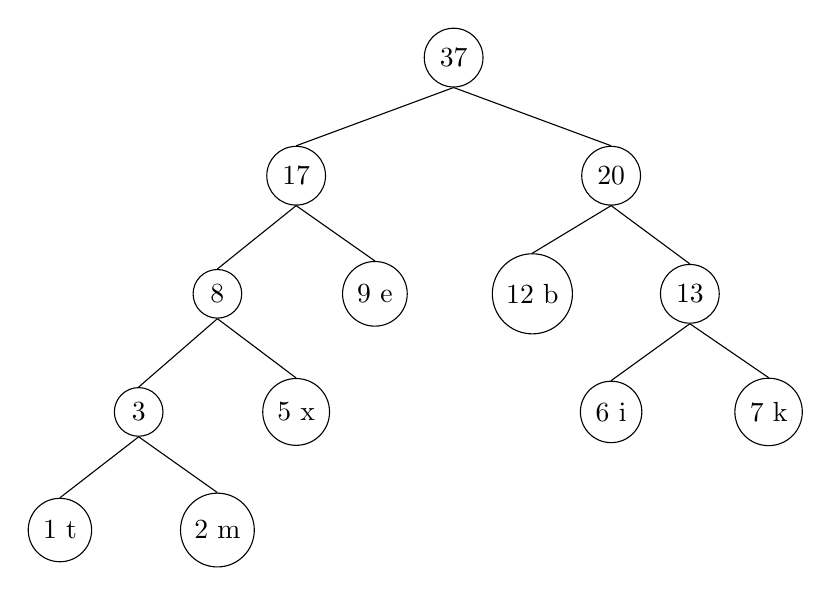
\begin{tikzpicture}[level distance=1.5cm,
                    level 1/.style={sibling distance=4cm},
                    level 2/.style={sibling distance=2cm},
                    every node/.style = {draw, circle}]
                \node {37}
                child { node {17}
                        child { node {8}
                                child { node {3}
                                        child { node {1 t} }
                                        child { node {2 m} }
                                    }
                                child { node {5 x} }
                            }
                        child { node {9 e} }
                    }
                child { node {20}
                        child { node {12 b}}
                        child { node {13}
                                child { node {6 i} }
                                child { node {7 k} }
                            }
                    };
            \end{tikzpicture}
        \end{center}
    \end{solution}

    \part[2] Now you can "decompress" the encoded sequence and recover the original word you lost. Please write the original word below.

    \begin{solution} \\
        %\vfill
        The word is tieke.
    \end{solution}

\end{parts}

\newpage

\titledquestion{K-Merge}

Recall that in merge sort, we learned how to merge two sorted arrays into one in linear time. In this question, we want to design a function that merge $K$ sorted arrays into one.

For example, here are 3 sorted arrays:
\begin{align*}
     & 1,5,9   \\
     & 2,3,6,7 \\
     & 4,6,7,9
\end{align*}
and we want to merge them as:
\begin{align*}
     & 1,2,3,4,5,6,6,7,7,9,9
\end{align*}

In the following question, suppose the sum of the lengths of the $K$ arrys is $n$. Here, assume $K=\omega(1)$ and $\log K=o(\log n)$.

\begin{parts}
    \part[2] Alice does not merge $K$ arrays at once. Instead, she decides to merge 2 of them each time. If she randomly choose 2 arrays and merges them, what is the time complexity of her algorithm in the \textbf{worst case}? You don't need to justify your answer.
    \begin{solution}
        The time complexity is $\theta(Kn)$.
    \end{solution}

    \part[2] Recall that in \textbf{worst case} merging two sorted arrays with lengths $n_1$ and $n_2$ needs $n_1+n_2-1$ comparisons. Now Alice wants to minimize the worst case number of comparisons in her algorithm. How should she choose the two arrays each time? Which algorithm does this strategy coincides with? \textbf{Briefly} give your answer.
    \begin{solution}
        %\vspace{2cm}
        To minimize the times of comparisons, Alice can first merge two arrays with lengths
        which are relatively less. Since the worst case is hard to be avoided, we should
        minimize the number of $n_1$ and $n_2$. If Alice merge arrays from those with longer
        lengths, these lengths will be added for more times. Thus Alice should start with arrays
        with less lengths. \\
        This strategy coincides with Huffman coding. Huffman coding lets words which are used
        more have less space. In this case space is confirmed while which array will be chosen
        for more times is the major problem.
    \end{solution}

    \part[2] Bob designs an algorithm that merges the $K$ arrays at once by modifying the merge function in merge sort. Each time, he looks up to the front element in each array and finds the smallest one among them. Then he puts this element at the back of his answer array and pop it from its original array. What is the time complexity of Bob's algorithm? \textbf{Briefly} justify your answer.
    \begin{solution}
        %\vspace{4cm}
        We should find the minimun among $K$ numbers, and repeat that operation. The operation
        will be repeated for no more than $n$ times though the last few operations will find minimum
        among less numbers. So that the time complexity is $O(Kn)$.
    \end{solution}

    \part[3] Now you need to improve Bob's algorithm to a better time complexity. \textbf{Briefly} describe your algorithm in natural language and give the complexity of your algorithm. Please focus on how to find the smallest front element in a shorter time.
    \begin{solution}
        %\vspace{7cm}
        we can first construct a min-heap to find the minimum in $K$ numbers. Then we pop the
        root of the heap, and insert a new element which is the next one in original array,
        thus make the operations after the first find be $\theta(log(K))$. The time complexity
        of constructing a min-heap is $\theta(K)$. For the whole progress, the time complexity
        will be reduced to $\theta(log(K)n)$.
    \end{solution}

\end{parts}



\newpage

\titledquestion{BST with Duplicates}

In our lecture, we require each BST node stands for a single unique element. However, in this question we are talking about BST with duplicated elements. That is, we need to maintain how many identical elements are in the BST. Now, each node may stands for multiple elements with the same value, and we call it the \ttt{count} of a node. Here we assume the value is \ttt{int} type.

First we give the definition of our \ttt{Node} struct.

\begin{cpp}
    struct Node {
            int val;    // The value of the node.
            int sumCount;    // The number of all elements in the sub-tree
            Node *left, *right; //the left and right child.
        };
\end{cpp}

Note that \ttt{sumCount} stands for the number of all elements in the \textbf{entire sub-tree}, i.e. the sum of \ttt{count} in the entire sub-tree. You will see why we use this definition in the following questions.

For example, if root $r$ has two children $a$ and $b$, and neither $a$ nor $b$ has a child. Suppose $r\ttt{.count}=n_r$, $a\ttt{.count}=n_a$ and $b\ttt{.count}=n_b$. Then $r\ttt{.sumCount}=n_r+n_a+n_b$, $a\ttt{.sumCount}=n_a$, and $b\ttt{.sumCount}=n_b$.

\begin{parts}
    \part[3] After figuring out the definition of member variable \ttt{sumCount}, you need to design a function that calculates the \ttt{count} of a node, using \ttt{sumCount} variable. Please complete this function below, and make sure you do not access \ttt{nullptr}.

    \begin{cpp}
        // return how many elements a single node stands for
        int get_count(Node *a){
                if(a == nullptr)
                return 0;
                int ans = /* (1) */ ;
                if(a->left != nullptr)
                /* (2) */ ;
                if(a->right != nullptr)
                /* (3) */ ;
                return ans;
            }
    \end{cpp}

    \begin{solution}
        %\vspace{3cm}
        \begin{enumerate}
            \item a$->$sumCount
            \item ans -= a$->$left$->$sumCount
            \item ans -= a$->$right$->$sumCount
        \end{enumerate}
    \end{solution}


    \part[4] Given a value $v$, we want to figure out how many elements are no more than $v$. Complete the function below, and make sure you do not access \ttt{nullptr}. You may use \ttt{get\_count} function if needed.
    By calling \ttt{count\_no\_more\_than(root, v)}, we can get the number of such elements in the entire BST.

    \begin{cpp}
        // return how many elements are no more than v.
        int count_no_more_than(Node *a, int v){
                if(a == nullptr)
                return 0;
                int ans = 0, tmp = 0;
                if (a->left != nullptr)
                tmp = /* (1) */ ;
                if(v < a->value)
                ans = /* (2) */ ;
                if(v == a->value)
                ans = /* (3) */ ;
                if(v > a->value)
                ans = /* (4) */ ;
                return ans;
            }
    \end{cpp}

    \begin{solution}
        %\vspace{3cm}
        \begin{enumerate}
            \item a$->$left$->$sumCount
            \item count\_no\_more\_than(a$->$left, v)
            \item tmp + a.get\_count()
            \item tmp + a.get\_count() + count\_no\_more\_than(a$->$right, v)
        \end{enumerate}
    \end{solution}


    \part[2] Now suppose you have finished the following two functions correctly. Given the root node of our BST, and two integers $l$ and $r$, how do you find out the number of elements in the range $[l,r]$? Use variables \ttt{root}, \ttt{l}, and \ttt{r}, and function \ttt{count\_no\_more\_than} to write an expression that computes the desired number.

    \begin{cpp}
        count_in_l_to_r = /* Your code */ ;
    \end{cpp}

    \begin{solution} \\
        %\vspace{1cm}
        count\_no\_more\_than(root, r) - count\_no\_more\_than(root, l-1)
    \end{solution}

    \part[3] \textbf{True or False}

    \begin{enumerate}
        \item[(i)] If we insert an element into our BST with duplicates, we may need to modify multiple nodes.
            \begin{oneparcheckboxes}
                \CorrectChoice True
                \choice False
            \end{oneparcheckboxes}

        \item[(ii)] If we delete a node in our BST with duplicates, the nodes that we need to modify are the nodes on the path from this node to the root.
            \begin{oneparcheckboxes}
                \CorrectChoice True
                \choice False
            \end{oneparcheckboxes}

        \item[(iii)] If we use member variable \ttt{count} instead of \ttt{sumCount}, we can still run \ttt{count\_no\_more\_than} in $O(h)$ time, where $h$ is the height of the tree.
            \begin{oneparcheckboxes}
                \choice True
                \CorrectChoice False
            \end{oneparcheckboxes}
    \end{enumerate}



\end{parts}

\end{questions}

\end{document}